The scope of the following measurement with dual-labeled \gls{dsDNA} is the analysis of the dependency of $\left\langle \tau_d \right\rangle$, $\left\langle N \right\rangle$, and $\left\langle MB \right\rangle$ on the brightness threshold $n_{br}$. The theoretically derived mathematical expressions from Section~\ref{Section:DerivedQuantities} are compared with the experimental findings.

\section{Measurement} \label{Section:BTCCD_Measurement_Dependencies}

A measurement of \SI{40}{\min} with dual-labeled \gls{dsDNA} was conducted. The recorded macro time trace was transformed into an \gls{IPL} time trace, and \gls{BTCCD} was applied according to the procedure described in Section~\ref{Section:DeterminationOfCoincidenceFraction}. Information on the burst threshold, the background, and on the starting parameters can be found in Table~\ref{Table:Measurement_dlDNA}. Since bursts are defined using the smoothed \gls{IPL} time trace, a burst may consist of only zero or one detected photon. For those bursts, no physically meaningful dwell time exists. To characterize the measurement only with stable bursts, the given values for $\left\langle \tau_d \right\rangle$, $\left\langle N \right\rangle$, and $\left\langle MB \right\rangle$ in the table are calculated from all bursts that contain at least three photons. This convention is used for the rest of the thesis, every time general information on a measurement is given.

\begin{table}[h]
		\centering
		\begin{tabular}{c|c|c|c|c|c} 
			ch. & $IPL^{thr}$ [\si{\micro\second}] & $\left\langle IPL^{bg} \right\rangle$ [\si{\micro\second}] & $\left\langle N \right\rangle$ [$10^{-3}$] & $\left\langle \tau_d \right\rangle$ [\si{\micro\second}] & $\left\langle MB \right\rangle$ [\si{\kilo\hertz}] \\
			\hline
			red & \num{150} & \num{794} & \num{10.19 +- 0.10} & \num{1123.6 +- 8.1} & \num{29.8 +- 4.1} \\
			blue & \num{180} & \num{1995} & \num{2.469 +- 0.040} & \num{844.7 +- 8.9} & \num{23.1 +- 7.8} \\
		\end{tabular}
	\caption[Burst threshold, background, and starting parameters for measurement of dual-labeled \gls{dsDNA}]{Burst threshold, background, and starting parameters for a measurement of \SI{40}{\min} with dual-labeled \gls{dsDNA}.}
	\label{Table:Measurement_dlDNA}
\end{table}

\section{Results}

\subsection{Dwell Time} \label{Section:PropertiesDwellTime}

A theoretical consideration came to the result that the dwell time $\left\langle \tau_d \right\rangle$ depends linearly on the brightness threshold $n_{br}$. Thus, the starting point of the analysis of the dwell time is a linear function
\begin{equation}
	\left\langle \tau_d \right\rangle (n_{br}) = \tau_d^0 + \Delta t_{\gamma} \cdot n_{br},
\end{equation}
where $\Delta t_{\gamma}$ and $\tau_d^0$ are fit parameters. The red dots in the upper graph of Figure~\ref{fig:CheckDependencies_DwellTimeRed_Theory} show the raw data for the red channel as well as a linear fit, illustrated by a green line. Underneath, in the lower graph, the corresponding residuals are plotted. As expected, the part of the raw data for smaller $n_{br}$ is not linear. Thus, the vertical dashed line indicates the interval that was used for fitting. For higher $n_{br}$, the linear function reflects the general increasing trend of the dwell time. Nonetheless, the residual plot reveals a structured deviation of the fit from the raw data.\\

In the figure, the values of the fit parameters are given. Additionally, the statistical measures $\chi^2/ n_{dof}$ and $p$ are stated. In general, $\chi^2$ is defined as
\begin{equation}
	\chi^2 = \sum_{i=1}^{n} \frac{(y_i - f(x_i))^2}{\sigma_{y_i}^2},
\end{equation}
where $n$ is the number of raw data points $(x_i, y_i)$ with uncertainty $\sigma_{y_i}$, and $f$ is the fitted model function. $\chi^2$ quantifies the deviation of the fit from the raw data in relation to the uncertainty. The value of $\chi^2$ follows the $\chi^2$ distribution that has the expectation value $n_{dof}$, where $n_{dof}$ is the difference between the number of measurement points $n$ and the parameters of the fit model. The normalization of $\chi^2$ on $n_{dof}$ allows an interpretation of the calculated value, and an evaluation of the fit quality. $p$ is the probability to obtain a value of $\chi^2$ that is larger than the calculated one.

\begin{figure}[h]
	\centering
	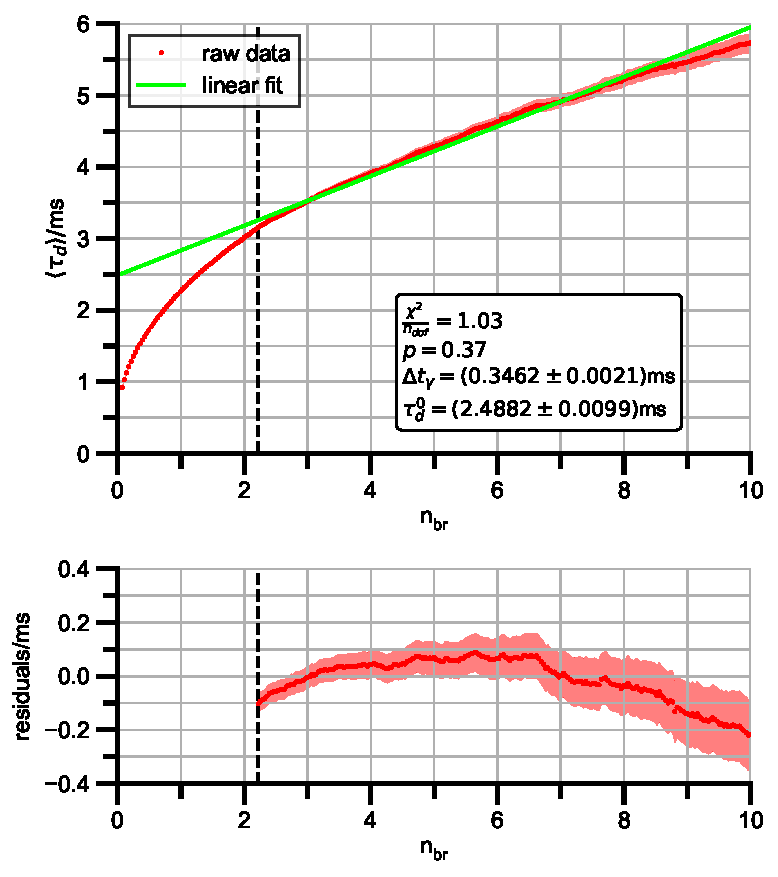
\includegraphics[width=4in]{CheckDependencies_DwellTimeRed_Theory.pdf}
	\caption[Linear fit of dwell time for red channel]{Linear fit according to $\left\langle \tau_d \right\rangle (n_{br}) =  \tau_d^0 + \Delta t_{\gamma} \cdot n_{br}$ for the red channel. The vertical dashed line indicates the range of $n_{br}$ that was used for fitting. For smaller $n_{br}$, the dependency is not linear. For higher $n_{br}$, the residual plot reveals a structure in the deviation of the fitted model from the raw data.}
	\label{fig:CheckDependencies_DwellTimeRed_Theory}
\end{figure}

The linear fit of the dwell time for the blue channel can be found in Figure~\ref{fig:CheckDependencies_DwellTimeBlue_Theory}. Table~\ref{Table:DwellTimeTheory} gives an overview of the fit parameters of the linear model for both channels.

\clearpage

\begin{table}[h!]
	\centering
	\begin{tabular}{c|c|c} 
		ch. & $ \tau_d^0$ [\si{\micro\second}] & $\Delta t_{\gamma}$ [\si{\micro\second}]  \\
		\hline
		red & \num{2488.2 +- 9.9} & \num{346.2 +- 2.1} \\
		blue & \num{1221 +- 17} & \num{381.7 +- 4.4} \\
	\end{tabular}
	\caption[Parameters of linear fit of dwell time]{Parameters of the fit of $\left\langle \tau_d \right\rangle (n_{br}) = \tau_d^0 + \Delta t_{\gamma} \cdot n_{br}$ for both channels.}
	\label{Table:DwellTimeTheory}
\end{table}

The part for smaller $n_{br}$ and the deviation revealed by the residual plot motivate a biexponential approach
\begin{equation}
	\left\langle \tau_d \right\rangle (n_{br}) = \tau_d^0 + \Delta \tau_1 (1 - e^{-n_{br}/ n_1}) + \Delta \tau_2 (1 - e^{-n_{br}/ n_2}),
\end{equation}
where $\tau_d^0$, $\Delta \tau_1$, $n_1$, $\Delta \tau_2$, and $n_2$ are fit parameters. The fit of this model for the red channel can be found in Figure~\ref{fig:CheckDependencies_DwellTimeRed_Experiment}. The biexponential function takes two different saturation processes into account that describe the dependency for the complete range of $n_{br}$ accurately. The fit for the blue channel is illustrated in Figure~\ref{fig:CheckDependencies_DwellTimeBlue_Experiment}.

\begin{figure}[h]
	\centering
	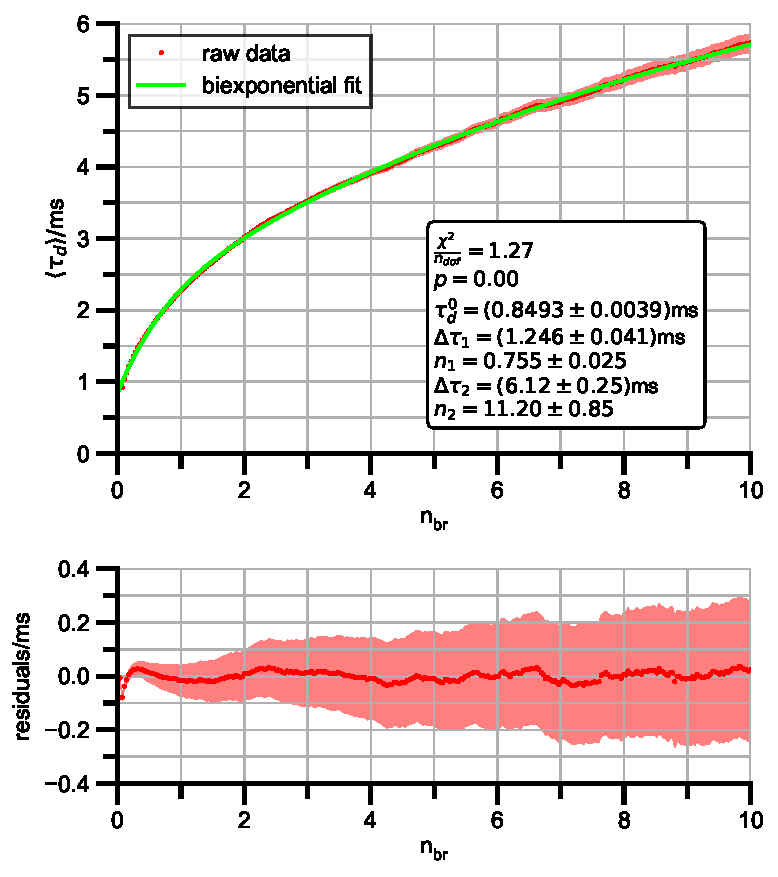
\includegraphics[width=4in]{CheckDependencies_DwellTimeRed_Experiment.pdf}
	\caption[Biexponential fit of dwell time for red channel]{Biexponential fit according to $\left\langle \tau_d \right\rangle (n_{br}) = \tau_d^0 + \Delta \tau_1 (1 - e^{-n_{br}/ n_1}) + \Delta \tau_2 (1 - e^{-n_{br}/ n_2})$ for the red channel. The biexponential function takes two different saturation processes into account. Thus, the residual plot does not show a structure anymore.}
	\label{fig:CheckDependencies_DwellTimeRed_Experiment}
\end{figure}
\clearpage
In Table~\ref{Table:DwellTimeExperiment}, the fit parameters for both channels are stated. They reveal that the exponential term modulated by $\Delta \tau_1$ and $n_1$ describes the initial saturation for smaller $n_{br}$, wherein a small range of $n_1$ the initial dwell time $\tau_d^0$ is increased by $\Delta \tau_1$. The second exponential term modulates an increase of the dwell time over a larger range of $n_2$. For the red channel, both exponential terms describe a saturation with notable effects in the relevant range of $n_{br}$ from $0$ to $10$. For the blue channel, the second exponential saturation takes places over an extremely large range of $n_2 = \num[{scientific-notation = true, separate-uncertainty = true}]{97(11)e5}$. Here, in fact, the second term describes a linear increase. Mathematically, this becomes obvious by rewriting it as
\begin{equation}
\Delta \tau_2 (1 - e^{-n_{br}/ n_2}) \approx \Delta \tau_2 (1 - (1 + n_{br}/ n_2)) = \frac{\Delta \tau_2}{n_2} n_{br},
\end{equation}
where $e^x \approx 1 + x$ for $x << 1$ was used. The slope is given by
\begin{equation}
m_2 = \frac{\Delta \tau_2}{n_2} = \SI{282 +- 49}{\micro\second},
\end{equation}
where the uncertainty was propagated according to
\begin{equation}
\sigma_{m_2} = m_2 \cdot \sqrt{\left(\frac{\sigma_{\Delta \tau_2}}{\Delta \tau_2}\right)^2 + \left(\frac{\sigma_{n_2}}{n_2}\right)^2}.
\end{equation}
$m_2$ can be compared with the results from the linear fit for the blue channel, where the slope was given by $\Delta t_{\gamma} = \SI{381.7 +- 4.4}{\micro\second}$, see Table~\ref{Table:DwellTimeTheory}. Both values are compatible with regard to their uncertainties:
\begin{equation}
\frac{\Delta t_{\gamma} - m_2}{\sqrt{\sigma_{m_2}^2 + \sigma_{\Delta t_{\gamma}}^2}} \approx \num{2.04}.
\end{equation}
The difference in the absolute values is a consequence of the different approaches. For the linear fit, the range of $n_{br}$ that was supposed to be linear was manually specified. By applying a biexponential fit, the range is mathematically optimized. Thus, the structure in the residuals, for the blue channel, reduces, compare Figures~\ref{fig:CheckDependencies_DwellTimeBlue_Theory} and \ref{fig:CheckDependencies_DwellTimeBlue_Experiment}.

\begin{table}[h]
	\centering
	\begin{tabular}{c|c|c|c|c|c} 
		ch. & $ \tau_d^0$ [\si{\micro\second}] & $\Delta \tau_1$ [\si{\micro\second}] & $n_1$ & $\Delta \tau_2$ [\si{\micro\second}] & $n_2$ \\
		\hline
		red & \num{849.3 +- 3.9} & \num{1246 +- 41} & \num{0.755 +- 0.025} & \num{6120 +- 250} & \num{11.20 +- 0.85} \\
		blue & \num{602.9 +- 4.8} & \num{1350 +- 140} & \num{2.47 +- 0.22} & \num[{scientific-notation = true, separate-uncertainty = true}]{274(35)e7} & \num[{scientific-notation = true, separate-uncertainty = true}]{97(11)e5} \\
	\end{tabular}
	\caption[Parameters of biexponential fit of dwell time]{Parameters of the fit of $\left\langle \tau_d \right\rangle (n_{br}) = \tau_d^0 + \Delta \tau_1 (1 - e^{-n_{br}/ n_1}) + \Delta \tau_2 (1 - e^{-n_{br}/ n_2})$ for both channels.}
	\label{Table:DwellTimeExperiment}
\end{table}

To sum it up, the theoretically derived linear expression allows a description of the increasing trend of $\left\langle \tau_d \right\rangle $ for larger values of $n_{br}$. However, a biexponential approach modulates the development of the dwell time over the complete range of $n_{br}$ accurately. The two exponential terms reveal two underlying processes. The first exponential saturation on a small range of $n_1$ can be explained by the exclusion of dim bursts, as already discussed in the theoretical derivation. In contrast, the second saturation on a larger scale $n_2$ does not necessarily take place in the relevant range of $n_{br}$, as observed for the blue channel. Its specific source is unknown.

\subsection{Number of Molecules}
The result of the theoretical derivation was that the average number of molecules inside the confocal detection volume $\left\langle N \right\rangle$ can be described by an exponential decay
\begin{equation}
	\left\langle N \right\rangle (n_{br}) = N^0e^{-n_{br}/ n},
\end{equation}
where $N^0$ and $n$ are fit parameters. Figure~\ref{fig:CheckDependencies_NumberMoleculesRed_Theory} shows the raw data and a fit of this model for the red channel. The fit reflects the general decreasing trend of $\left\langle N \right\rangle$, but deviates significantly from its specific behavior. A similar effect can be observed for the blue channel, see Figure~\ref{fig:CheckDependencies_NumberMoleculesBlue_Theory}. An overview of the fit parameters for both channels is given in Table~\ref{Table:NumberMoleculesTheory}.

\begin{figure}[h!]
	\centering
	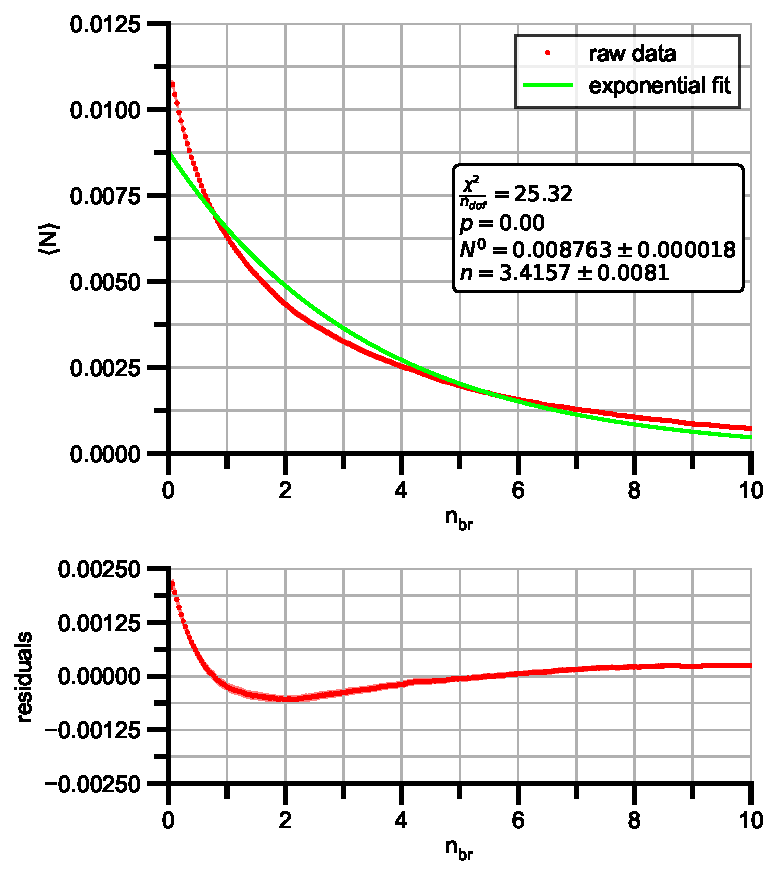
\includegraphics[width=4in]{CheckDependencies_NumberMoleculesRed_Theory.pdf}
	\caption[Exponential fit of molecule number for red channel]{Exponential fit according to $\left\langle N \right\rangle (n_{br}) = N^0e^{-n_{br}/ n}$ for the red channel. The fit reflects the general decreasing trend of $\left\langle N \right\rangle$, but deviates clearly from the specific behavior.}
	\label{fig:CheckDependencies_NumberMoleculesRed_Theory}
\end{figure}

\begin{table}[h!]
	\centering
	\begin{tabular}{c|c|c} 
		ch. & $N^0$ [$10^{-3}$] & $n$ \\
		\hline
		red & \num{8.763 +- 0.018} & \num{3.4157 +- 0.0081} \\
		blue & \num{2.680 +- 0.013} & \num{2.178 +- 0.011} \\
	\end{tabular}
	\caption[Parameters of exponential fit of molecule number]{Parameters of the fit of $\left\langle N \right\rangle (n_{br}) = N^0e^{-n_{br}/ n}$ for both channels.}
	\label{Table:NumberMoleculesTheory}
\end{table}
\clearpage
An improved model has to take the deviation between the theoretically derived expression and the raw data into account. The average number of molecules inside the confocal detection volume is directly calculated from the dwell time, see Equation~\eqref{Equation:AverageNumberOfMolecules}. Thus, inspired by the two processes observed for the dwell time above, a biexponential decay 
\begin{equation}
	\left\langle N \right\rangle (n_{br}) = ae^{-n_{br}/ n_1} + be^{-n_{br}/ n_2}
\end{equation}
is proposed. Here, $a$, $n_1$, $b$, and $n_2$ are the fit parameters. A fit of this function for the red channel can be found in Figure~\ref{fig:CheckDependencies_NumberMoleculesRed_Experiment}. The biexponential model describes the data more accurately than the monoexponential function. This is also reflected in the residual plot. The results for the blue channel show the same improvement and can be found in Figure~\ref{fig:CheckDependencies_NumberMoleculesBlue_Experiment}. Table~\ref{Table:NumberMoleculesExperiment} contains the fit parameters for both the blue and the red channel. The parameters reveal again that the first exponential decay modulates a decrease of $\left\langle N \right\rangle$ by $a$ over a relative short range $n_1$. The second exponential term describes a decay by $b$ over a larger range $n_2$. In contrast to the dwell time in the previous section, here, the second exponential decay with reasonable values for $b$ and $n_2$ can be observed in both channels.

\begin{figure}[h!]
	\centering
	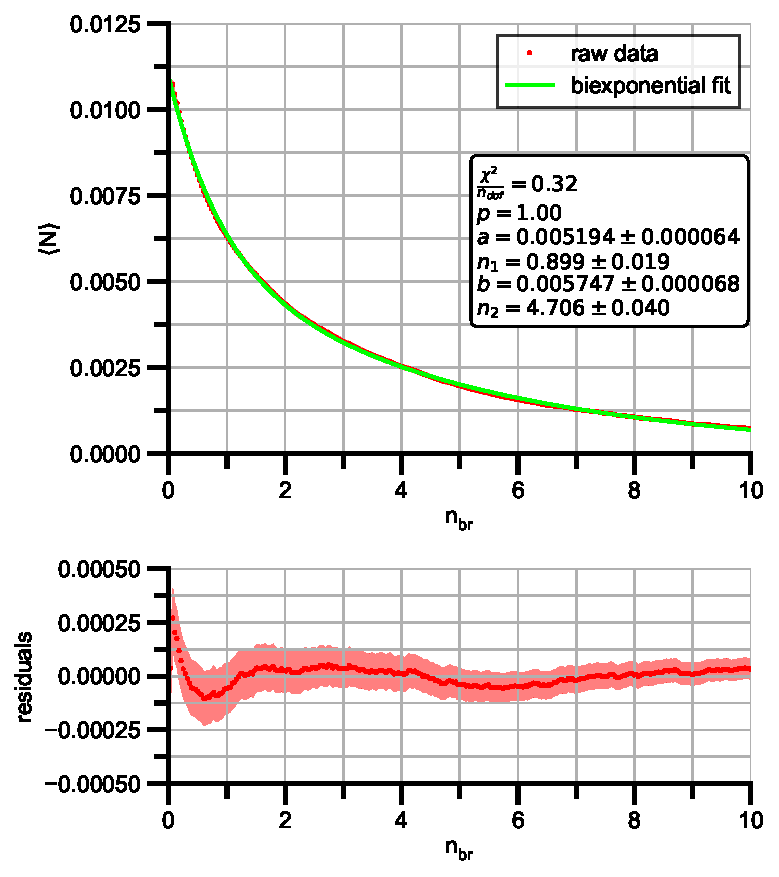
\includegraphics[width=4in]{CheckDependencies_NumberMoleculesRed_Experiment.pdf}
	\caption[Biexponential fit of molecule number for red channel]{Biexponential fit according to $\left\langle N \right\rangle (n_{br}) = ae^{-n_{br}/ n_1} + be^{-n_{br}/ n_2}$ for the red channel. The two decay processes of the biexponential function modulate the measurement more accurately than the monoexponential model.}
	\label{fig:CheckDependencies_NumberMoleculesRed_Experiment}
\end{figure}
\clearpage
\begin{table}[h!]
	\centering
	\begin{tabular}{c|c|c|c|c} 
		ch. & $a$ [$10^{-3}$] & $n_1$ & $b$ [$10^{-3}$] & $n_2$ \\
		\hline
		red & \num{5.194 +- 0.064} & \num{0.899 +- 0.019} & \num{5.747 +- 0.068} & \num{4.706 +- 0.040} \\
		blue & \num{1.38 +- 0.15} & \num{1.163 +- 0.094} & \num{1.53 +- 0.16} & \num{2.82 +- 0.11} \\
	\end{tabular}
	\caption[Parameters of biexponential fit of molecule number]{Parameters of the fit of $\left\langle N \right\rangle (n_{br}) = ae^{-n_{br}/ n_1} + be^{-n_{br}/ n_2}$ for both channels.}
	\label{Table:NumberMoleculesExperiment}
\end{table}

In conclusion, a biexponential decay describes the average number of molecules inside the confocal detection volume $\left\langle N \right\rangle$ accurately. The analysis yields again two processes that lead to a decrease of $\left\langle N \right\rangle$. In contrast to the results for the dwell time above, they are observable for both channels.

\subsection{Molecular Brightness}

The theoretical consideration obtained that an exponential saturation 
\begin{equation}
	\left\langle MB \right\rangle (n_{br})   = MB^0 + \Delta MB(1 - e^{-n_{br}/ n}),
\end{equation}
where $MB^0$, $\Delta MB$, and $n$ are fit parameters, describes the molecular brightness. The raw data and a fit for the red channel can be found in Figure~\ref{fig:CheckDependencies_MolecularBrightnessRed_Theory}. Over large parts, the monoexponential model describes the raw data correctly. However, for $n_{br} < 1$, it underestimates the increasing trend of the raw data. The fit for the blue channel can be found in Figure~\ref{fig:CheckDependencies_MolecularBrightnessBlue_Theory}. For the blue channel, such a deviation is not observed. The low $\chi^2/ n_{dof}$ for both channels is a result of the relatively large uncertainty on the molecular brightness. Since $\left\langle MB \right\rangle$ is an average value calculated from all bursts, it is a sensitive quantity. The extreme uncertainty for $n_{br} \rightarrow 0$ comes from bursts with only a tiny number of photons. This is another reason, why, for the characterization of the measurement above, a minimal number of at least three photons was required. The fit parameters for both channels are stated in Table~\ref{Table:MolecularBrightnessTheory}.\\

Despite the broad agreement of the monoexponential fit with the raw data, a biexponential model
\begin{equation}
\left\langle MB \right\rangle (n_{br}) = MB^0 + \Delta MB_1(1 - e^{-n_{br}/ n_1}) + \Delta MB_2(1 - e^{-n_{br}/ n_2}),
\end{equation}
where $MB^0$, $\Delta MB_1$, $n_1$, $\Delta MB_2$, and $n_2$ are the parameters, is fitted. Hereby, it is investigated if the two processes that were observed for the dwell time and the number of molecules are also present in the molecular brightness. Figure~\ref{fig:CheckDependencies_MolecularBrightnessRed_Experiment} illustrates the fit for the red channel. The fit for the blue channel is depicted in Figure~\ref{fig:CheckDependencies_MolecularBrightnessBlue_Experiment}. As expected, the value of $\chi^2/ n_{dof}$ becomes even lower. However, for the red channel, the biexponential fit modulates the part of the raw data for $n_{br} < 1$ more precisely than the monoexponential saturation. The fit parameters reveal two distinct processes described by the two exponential functions, as can be seen in Table~\ref{Table:MolecularBrightnessExperiment}. For the blue channel, the parameters of the second exponential saturation with regard to their large uncertainties are in agreement with zero. Therefore, the molecular brightness is effectively described by a monoexponential saturation. The situation for the blue channel is similar to the results for the dwell time, where the second process is not as much pronounced as in the red channel.


\vfill
\begin{figure}[h]
	\centering
	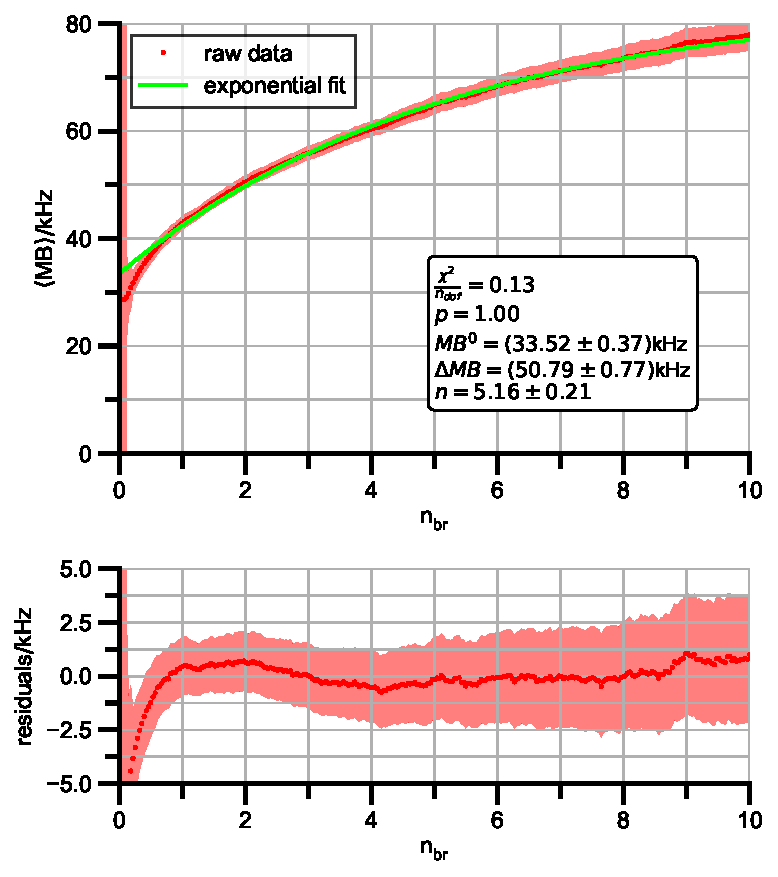
\includegraphics[width=4in]{CheckDependencies_MolecularBrightnessRed_Theory.pdf}
	\caption[Exponential fit of molecular brightness for red channel]{Exponential fit according to $\left\langle MB \right\rangle (n_{br}) = MB^0 + \Delta MB(1 - e^{-n_{br}/ n})$ for the red channel. For ${n_{br} < 1}$, the model  slightly underestimates the increasing trend of the raw data. The comparably large uncertainty on $\left\langle MB \right\rangle$ explains the low value for $\chi^2/ n_{dof}$ for the fits.}
	\label{fig:CheckDependencies_MolecularBrightnessRed_Theory}
\end{figure}
\vfill
\begin{table}[h]
	\centering
	\begin{tabular}{c|c|c|c} 
		ch. & $MB^0$ [\si{\kilo\hertz}] & $\Delta MB$ [\si{\kilo\hertz}] & $n$ \\
		\hline
		red & \num{33.52 +- 0.37} & \num{50.79 +- 0.77} & \num{5.16} \\
		blue & \num{23.39 +- 0.63} & \num{12.8 +- 2.3} & \num{7.53 +- 2.87} \\
	\end{tabular}
	\caption[Parameters of exponential fit of molecular brightness]{Parameters of the fit of $\left\langle MB \right\rangle (n_{br}) = MB^0 + \Delta MB(1 - e^{-n_{br}/ n})$ for both channels.}
	\label{Table:MolecularBrightnessTheory}
\end{table}

\clearpage

\vspace*{\fill}
\begin{figure}[h]
	\centering
	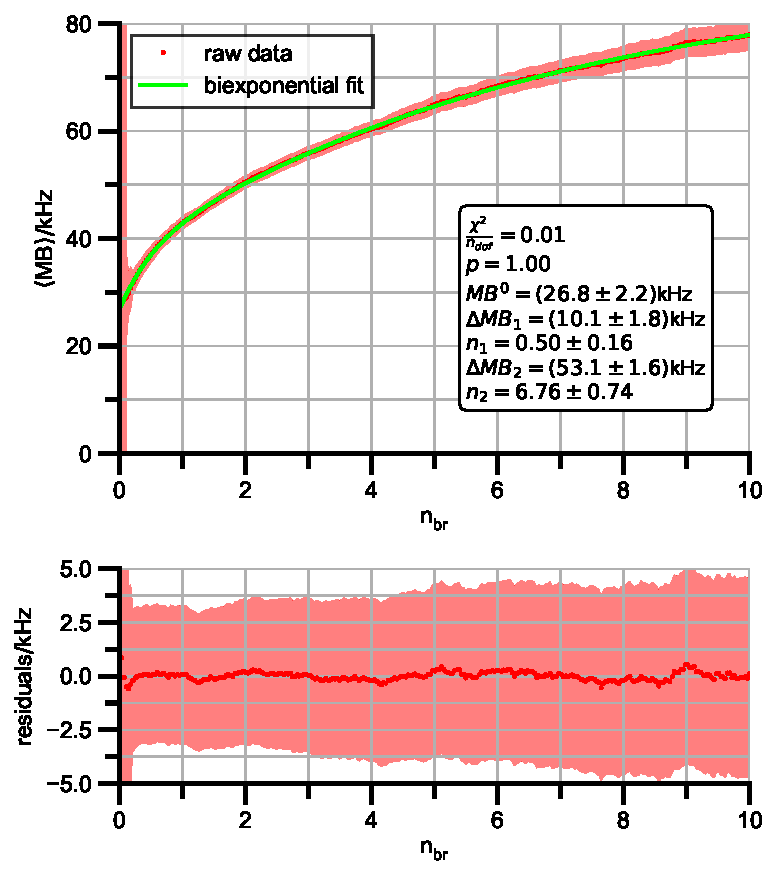
\includegraphics[width=4in]{CheckDependencies_MolecularBrightnessRed_Experiment.pdf}
	\caption[Biexponential fit of molecular brightness for red channel]{Fit according to $\left\langle MB \right\rangle (n_{br}) = MB^0 + \Delta MB_1(1 - e^{-n_{br}/ n_1}) + \Delta MB_2(1 - e^{-n_{br}/ n_2})$ for the red channel. Information on the measurement can be found in Section~\ref{Section:BTCCD_Measurement_Dependencies}. The biexponential model describes the part of the raw data for $n_{br} < 1$ with a higher slope more precisely than the monoexponential approach.}
	\label{fig:CheckDependencies_MolecularBrightnessRed_Experiment}
\end{figure}
\vspace*{\fill}
\begin{table}[h]
	\centering
	\begin{tabular}{c|c|c|c|c|c} 
		ch. & $MB^0$ [\si{\kilo\hertz}] & $\Delta MB_1$ [\si{\kilo\hertz}] & $n_1$ & $\Delta MB_2$ [\si{\kilo\hertz}] & $n_2$ \\
		\hline
		red & \num{26.8 +- 2.2} & \num{10.1 +- 1.8} & \num{0.50 +- 0.16} & \num{53.1 +- 1.6} & \num{6.76 +- 0.74} \\
		blue & \num{19.7 +- 3.6} & \num{6.0 +- 3.2} & \num{0.84 +- 0.50} & \num[{scientific-notation = true, separate-uncertainty = true}]{-13(21)e6} & \num[{scientific-notation = true, separate-uncertainty = true}]{-17(27)e6} \\
	\end{tabular}
	\caption[Parameters of biexponential fit of molecular brightness]{Parameters of a fit of $\left\langle MB \right\rangle (n_{br}) = MB^0 + \Delta MB_1(1 - e^{-n_{br}/ n_1}) + \Delta MB_2(1 - e^{-n_{br}/ n_2})$ for both channels.}
	\label{Table:MolecularBrightnessExperiment}
\end{table}
\vspace*{\fill}

\clearpage

Overall, for the red channel, two processes are observed. Hence, a biexponential saturation describes the raw data more accurately than a monoexponential model. For the blue channel, the second process is not very pronounced. The uncertainty on $\left\langle MB \right\rangle$ complicates the specification of the raw data for higher values of $n_{br}$. 

\section{Two Underlying Processes}

In the previous section, it was shown phenomenologically that the dependency of $\left\langle \tau_d \right\rangle$, $\left\langle N \right\rangle$, and $\left\langle MB \right\rangle$ on the brightness threshold $n_{br}$ can be modulated by two distinct exponential terms. For $\left\langle \tau_d \right\rangle$ and $\left\langle MB \right\rangle$, a biexponential saturation takes place, while $\left\langle N \right\rangle$ is described by a biexponential decay. The two exponential terms of the form $e^{-n_{br}/ n_1}$ and $e^{-n_{br}/ n_2}$ represent two processes that have an influence on the \gls{BTCCD} analysis. Table~\ref{Table:TwoProcesses} gives an overview of the ranges $n_1$ and $n_2$ for all analyzed quantities. The first exponential term describes a process over a small range of $n_{br}$, while the second process takes place over a larger range. The specific range varies for every quantity, and, for the blue channel, the second process is less pronounced.

\begin{table}[h]
	\centering
	\begin{tabular}{c|c|c|c} 
		ch. & quantity & $n_1$ & $n_2$  \\
		\hline
		\multirow{3}{*}{red} & $\left\langle \tau_d \right\rangle$ & \num{0.755 +- 0.025} & \num{11.20 +- 0.85}\\
		& $\left\langle N \right\rangle$ & \num{0.899 +- 0.019} & \num{4.706 +- 0.040}\\
		& $\left\langle MB \right\rangle$ & \num{0.50 +- 0.16} & \num{6.76 +- 0.74}\\
		\hline
		\multirow{3}{*}{blue} & $\left\langle \tau_d \right\rangle$ & \num{2.47 +- 0.22} & \num[{scientific-notation = true, separate-uncertainty = true}]{97(11)e5}\\
		& $\left\langle N \right\rangle$ & \num{1.163 +- 0.094} & \num{2.82 +- 0.11}\\
		& $\left\langle MB \right\rangle$ & \num{0.84 +- 0.50} & \num[{scientific-notation = true, separate-uncertainty = true}]{-17(27)e6}
	\end{tabular}
	\caption[Ranges of two underlying processes]{Overview of the ranges of the exponential terms of the form $e^{-n_{br}/ n_1}$ and $e^{-n_{br}/ n_2}$ that describe the analyzed quantities.}
	\label{Table:TwoProcesses}
\end{table}

The first process is the exclusion of dim bursts connected with peripheral and borderline trajectories. 

The second process allows the conclusion that another phenomenon in the order of the dwell time takes place during the measurement. This process changes the fluorescence characteristic. Transitions to triplet states, see Section~\ref{Section:Fluorescence}, increase the average time that an excited electron takes to relax into the ground state and to emit a photon. The occurrence of triplet state transitions depends on the chemical structure of the dye and the intensity of the incoming laser light \cite{Lakowicz2006}. Thus, the variation of the intensity is a way to investigate the origin of the second term further. Another aspect is the negative charge of DNA. In combination with the overall positive charge of Atto 647N and the negative charge of Alexa 488, Coulomb interactions could influence the fluorescence emission of the dyes \cite{ZanettiDomingues2013}. 

There is a variety of other processes that change the emission characteristics of a fluorophore. Hence, the specific nature of the second process is an object of further research \cite{Bielec2020}.